\section{Data taking}
%
The results reported here are based on data taken in October 2012 
in a dedicated LHC proton fill (3216)
with very special beam properties. The beam optics with $\beta^{*} = 1000\,$m
has been specifically developed for measuring low-$|t|$ elastic scattering.
Like the previously used $\beta^{*} = 90\,$m optics~\cite{epl96,epl101-tot,prl111},
this new optics configuration
provides parallel-to-point focussing in the vertical plane at the RP position 
$s = 220\un{m}$, implemented by tuning the transport matrix elements via the
LHC magnet currents: the magnification $v_{y}$ is made to vanish whereas the 
effective length $L_{y}$ is maximised ($285.6\un{m}$ as compared to $260\un{m}$ for 
$\beta^{*} = 90\,$m).
The resulting large displacement of a scattered proton with a given $t$-value 
away from the beam centre at the RP, together with a very small beam 
divergence in the interaction point and hence a tiny beam width 
at the RP ($\sigma_{y} = 260\,\mu$m as compared to 700\,$\mu$m for 
$\beta^{*} = 90\,$m) translates into 
an acceptance for $|t|$-values down to $10^{-4}\,\rm GeV^{2}$, provided the 
vertical RPs can approach the beam centre to only a few nominal beam standard 
deviations~\footnote{The nominal standard deviation is defined as 
the beam width for a normalised emittance 
$\varepsilon \gamma = 3.5\,\mu$m\,rad.}.
A further improvement relative to $\beta^{*} = 90\,$m is the non-vanishing 
effective length in the horizontal plane, $L_{x} = 46.8\,$m at $s = 220\,$m, 
enabling a better reconstruction of the horizontal component of the 
scattering angle.

The vertical RP approach to only $3\,\sigma_{y}$ from the beam centre required
low beam currents -- two colliding bunch pairs and in each beam one 
non-colliding bunch for background monitoring, with $10^{11}$ protons per bunch 
-- and a novel collimation strategy 
to keep the beam halo background under control. As a first step, the primary 
collimators (TCP) in LHC point 7 scraped the beam down to $2\,\sigma_{y}$; then 
they were retracted to $2.5\,\sigma_{y}$, thus creating a $0.5\,\sigma_{y}$ gap 
between
the beam edge and the collimator jaws. With the halo strongly suppressed 
and no collimator producing showers by touching the beam, the RPs at 
$3\,\sigma_{y}$ were operated in a background-depleted environment for about one 
hour until the beam-to-collimator gap was refilled by diffusion, as 
diagnosed by the increasing RP trigger rate (Figure~\ref{fig:overview}, top). As soon as the background conditions
had deteriorated to an unacceptable level, the beam cleaning procedure as described above was repeated, again followed by a quiet data-taking period.
This entire sequence was iterated 6 times until the luminosity had degraded 
from initially $2\times10^{27}\,\rm cm^{-2}s^{-1}$ to 
$0.5\times10^{27}\,\rm cm^{-2}s^{-1}$ \todo{(check!)} % mean value from data: 19.8E3 mb^-1 / 17 772 s ~ 1 mb^-1 s^-1 = 10^27 cm^-2 s^-1
at which point the data yield was considered as too low. 
During the 9 hour long fill, an integrated luminosity of $27\,\rm \mu b^{-1}$ 
\todo{($19.8$ used in data analysis)} has been  
accumulated, split into 6 data sets corresponding to the calm periods between
the cleaning operations. 

Due to an anti-collision protection system the top and the bottom pots of a 
vertical RP unit could not approach each other close enough to be both at a 
distance of $3\,\sigma_{y} = 780\,\mu$m from the beam centre. Therefore a 
configuration with one RP diagonal (top pots left of IP5 -- bottom pots right
of IP5) at $3\,\sigma_{y}$ and the other (bottom left -- top right) at 
$10\,\sigma_{y}$ was chosen. The far diagonal provides a systematic comparison
at larger $|t|$-values.
The horizontal RPs were less critical for this measurement and placed at a
safe distance of $10\,\sigma_{x} \approx 7.5$\,mm.

The collected events were triggered by a logical \textit{OR} of: inelastic 
trigger (activity in either arm of T1 or T2), double-arm proton trigger 
(coincidence of any RP left of IP5 and any RP right of IP5) and zero-bias trigger
(random bunch crossings) for calibration purposes.

\todo{190k (162k) elastic events tagged in close (far) diagonal}.


\begin{figure*}
\begin{center}
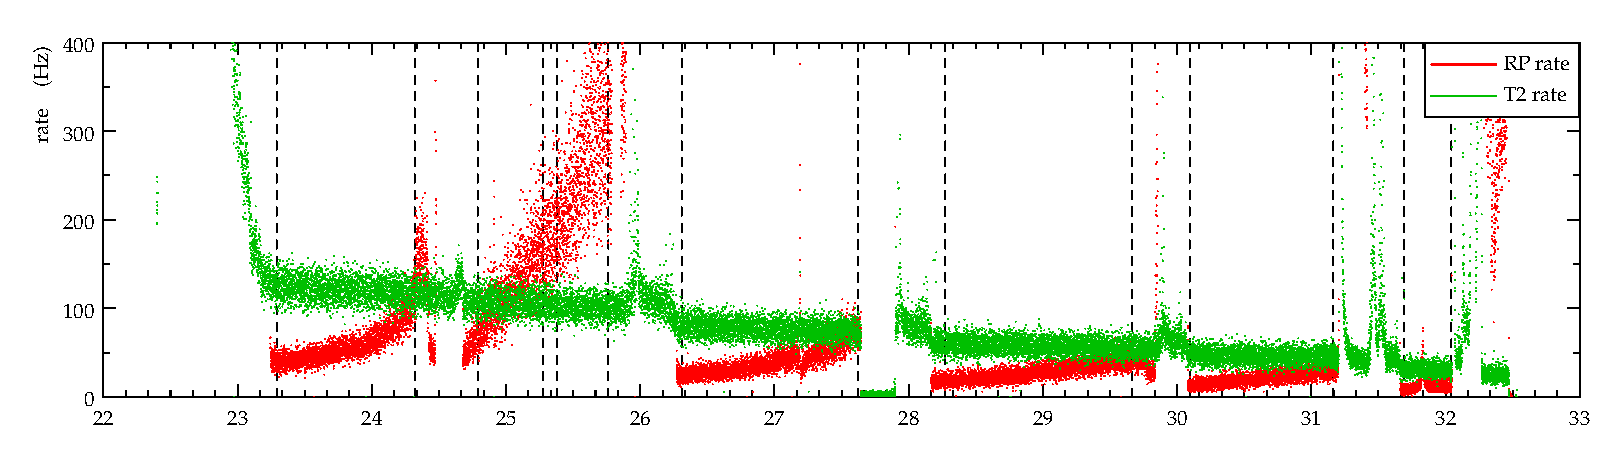
\includegraphics[width=16cm]{fig/overview.pdf}
\vskip-3mm
\caption{%
Illustration of the beam conditions. The T2 rate is roughly proportional to luminosity. The RP rate is sensitive to luminosity plus beam-halo.
%The pile-up probability follows the intensity of beam-halo protons.
}
\label{fig:overview}
\end{center}
\end{figure*}
